\section{One Hierarchy per Size}\label{sec:strees}
% 2026-09-21 the fair state-of-the-art section (house order): the tree of one size, its own nodes, the STrees layout
% and its cost, the per-size construction, and the closing remark that re-lists the three limitations.  Cadence pass.

This section describes the hierarchy of one size, the tree of its nuclei, and the index that stores one such tree per size.
%
The chain index of Sections~\ref{sec:chains} to~\ref{sec:construction} keeps the trees of every size and stores them differently.

\stitle{The tree of one size.}
Fix a size $s$.
%
Two nuclei of size $s$ are disjoint or nested.
%
Let $N$ be an $\Nuc{s}{k}$ and $N'$ an $\Nuc{s}{k'}$ with $k\le k'$, and let the two share a vertex.
%
Every vertex of $N\cup N'$ lies in at least $k$ cliques of $s$ vertices inside the union, and the union is connected through the shared vertex.
%
The union therefore satisfies the two properties of Definition~\ref{def:nucleus} at level $k$.
%
By the maximality of $N$, the union is $N$, and $N'\subseteq N$.
%
The nuclei of size $s$ therefore form a laminar family: any two are disjoint or nested.
%
One vertex set can be a nucleus for a whole interval of levels.
\begin{definition}[canonical node, own node]\label{def:node}
A \textit{canonical node} of size $s$ is a vertex set that is an $\Nuc{s}{k}$ for at least one level $k$.
%
Its \textit{top} is the largest such $k$.
%
The canonical nodes of size $s$ ordered by inclusion form the forest $\Tree{s}$: the largest sets are its roots, and a node's children are the largest nodes strictly inside it.
%
The \textit{own node} of a vertex $v$ with $\core{s}{v}\ge1$, denoted as $\own{s}{v}$, is the $\Nuc{s}{\core{s}{v}}$ containing $v$.
\end{definition}
% 2026-09-22 prose pass: the three facts about tops each carry their reason (nesting, maximality); the derived properties of the own node moved out of the definition.
The own node of $v$ is the deepest node of $\Tree{s}$ containing $v$, and its top is $\core{s}{v}$: a larger top would put $v$ in a nucleus of a larger level.
%
The top of a node equals the smallest core value of its vertices.
%
Otherwise every vertex of a node of top $t$ would have a core value above $t$, and its nucleus at level $t+1$ would lie inside the node by the nesting above.
%
Every vertex of the node would then lie in at least $t+1$ cliques of $s$ vertices inside the node.
%
The node would have the two properties at level $t+1$, and its top would exceed $t$.
%
Tops increase strictly from a root down to its descendants.
%
A node with top $t$ has the two properties at every level up to $t$, so a child, which is maximal at its own top, has a top above $t$.
%
The nodes containing $v$ are the path from $\own{s}{v}$ up to its root.
%
For $1\le k\le\core{s}{v}$, the community of $v$ at $(s,k)$ is therefore the highest node on this path whose top is at least $k$.
%
We call it the highest ancestor-or-self of $\own{s}{v}$ with top at least $k$.
\begin{figure}[t]
\centering
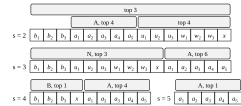
\includegraphics[width=\columnwidth]{figures/fig_strees.pdf}
\caption{\strees for Figure~\ref{fig:example}: the tree of every size over its depth-first array; a node is a bar over its slice.}
\label{fig:strees}
\end{figure}
\begin{example}\label{ex:tree}
Consider Figure~\ref{fig:example}; Figure~\ref{fig:strees} draws the trees of its four sizes.
%
At size $2$ the forest $\Tree{2}$ has one root holding all $15$ vertices.
%
The graph is connected and its smallest degree is $3$ (at $b_1$ and $b_2$), so the root is the $(2,k)$-nucleus for $k=1,2,3$ and has top $3$.
%
The root has two children of top $4$, $A$ and $\{x,u_1,\dots,w_3\}$.
%
At size $3$ the forest $\Tree{3}$ has two roots and no other node: $N=B\cup\{u_1,\dots,w_3\}$ with top $3$ and $A$ with top $6$.
%
No triangle joins them, because the edge $a_5b_3$ lies in none.
%
At size $4$ the roots are $A$ (top $4$) and $B$ (top $1$), and at size $5$ the forest is $A$ alone.
%
The own node of $b_1$ is the root at size $2$, $N$ at size $3$ and $B$ at size $4$.
%
The community of $x$ at $(2,3)$ is the root, the highest ancestor of $\own{2}{x}=\{x,u_1,\dots,w_3\}$ with top at least $3$.
\end{example}

\stitle{The index of one size.}
The tree of one size gives a fast index for that size~\cite{fastHierarchy,Fang2016CLtree}.
%
The vertices with $\core{s}{v}\ge1$ are written into one array in a depth-first traversal of $\Tree{s}$, each vertex when the traversal reaches its own node.
%
The vertices of every node then form one contiguous slice of the array, since the traversal visits a node and all its descendants before moving on.
%
In Figure~\ref{fig:strees} every node is drawn as a bar over its slice, and the vertices under a bar that no child bar covers are the node's own vertices.
%
Every node stores its top, its parent and the two ends of its slice.
%
Every vertex stores its own node and its core value.
%
A community query climbs from the own node to the highest ancestor whose top is at least $k$ and copies that node's slice.
%
A value query reads the stored value.
%
The answer is one memory copy.

\stitle{One hierarchy per size.}
Every size has its own tree.
%
The index for every size stores one tree and one array per size, together with every core value.
%
We call this index \strees and measure against it throughout.
%
A vertex $v$ appears in the arrays of the $\omg{v}-1$ sizes $2$ to $\omg{v}$.
%
The arrays therefore hold $\sum_v(\omg{v}-1)$ entries, $44$ cells for the $15$ vertices of Figure~\ref{fig:strees}.
%
There are as many own-node pointers, and as many stored values.
%
On \webuk a vertex lies in $181$ arrays on average, and \strees takes $190$~MB for $129{,}632$ vertices.
%
On a coauthorship graph whose largest cliques have $337$ vertices it takes $202$~MB for $540{,}486$ vertices, and on a coauthorship graph of $4$ million vertices it takes $506$~MB.
%
Building \strees means one decomposition per size.
%
With the counting-based decomposition \cnd~\cite{Zhang2026NucleusCounting}, the $499$ sizes of \webuk take $15.7$ hours of building and peeling.

\begin{remark}
\strees answers a community query with one memory copy, and it is the natural index for one size.
%
Across sizes it runs into the three difficulties of Section~\ref{sec:intro}.
%
\emph{Repetition across sizes}: a vertex is stored once per size it lives in.
%
\emph{Contiguity of communities}: a community is one block only inside its own size's array, and an index that groups vertices across sizes must make communities contiguous in another way.
%
\emph{Construction of every size}: each size is one decomposition.
%
The next sections keep its trees and its memory-copy answers and remove the repetition.
\end{remark}
